\documentclass{article}

\usepackage{booktabs}
\usepackage{color}
\usepackage{pgf}
\usepackage{tikz}
\usetikzlibrary{arrows,positioning,fit,shapes,decorations,decorations.pathmorphing,decorations.pathreplacing,calc,patterns,scopes,matrix}
\pgfrealjobname{parseapi}

\usepackage{helvet}
\usepackage{enumitem}
\usepackage[letterpaper]{geometry}
\usepackage{listings}
\usepackage{verbatim}
\usepackage[T1]{fontenc}

\setlength{\parindent}{0.0in}
\setlength{\parskip}{0.1in}

\newenvironment{apient}{\small\verbatim}{\endverbatim}

\newcommand{\apidesc}[1]{%
{\addtolength{\leftskip}{4em}%
#1\par\medskip}
}

\newcommand{\definedin}[1]{%
\textbf{Defined in:} \texttt{#1}
}

\begin{document}
\thispagestyle{empty}

\begin{titlepage}
\beginpgfgraphicnamed{titlepage}
\begin{tikzpicture}[remember picture, overlay]
    \path
        (current page.north west) coordinate (origin)
        (current page.north) coordinate (topcenter);

    % Header
    \node [font=\sffamily] (pppt) at ($(topcenter) - (0,1.0in)$) 
        {\fontsize{24}{36}\selectfont Paradyn Parallel Performance Tools};

    % Document Title
% older versions of pgf have a bug for matrices in overlay mode;
% have to specify positions manually
%    \matrix (Title) [%
%        matrix of nodes,%
%        nodes={font=\sffamily,right},%
%        matrix anchor=west,%
%        row sep=12pt
%        ] at ($(origin)+(0.75in,-3.0in)$)
%    {
%        \fontsize{48}{56}\selectfont ParseAPI \\
%        \fontsize{44}{56}\selectfont Programmer's Guide \\
%    };

    \node [anchor=west,font=\sffamily] (title1) at ($(origin)+(0.75in,-3.0in)$)
        {\fontsize{48}{56}\selectfont ParseAPI};
    \node [anchor=west,font=\sffamily] (title2) at ($(title1.west)+(0in,-56pt)$)
        {\fontsize{48}{56}\selectfont Programmer's Guide};

    % Release information
%    \matrix (Releaseinfo) [%
%        matrix of nodes,%
%        nodes={font=\sffamily,right},%
%        matrix anchor=west,%
%        row sep=8pt
%        ] at ($(origin)+(0.75in,-5.0in)$)
%    {
%        %\fontsize{24}{32}\selectfont Release 0.1 \\
%        \fontsize{24}{32}\selectfont Beta Release \\
%        \fontsize{24}{32}\selectfont Oct 2010 \\
%    };

    \node [anchor=west,font=\sffamily] (rel1) at ($(origin)+(0.75in,-5.0in)$)
        {\fontsize{24}{32}\selectfont 7. 0 Release};
    \node [anchor=west,font=\sffamily] (rel2) at ($(rel1.west)+(0in,-32pt)$)
        {\fontsize{24}{32}\selectfont Mar 2011};

    % Contact information
%    \matrix (UWaddress) [%
%        matrix of nodes,%
%        nodes={font=\sffamily\large,right},%
%        matrix anchor=north west
%        ] at ($(origin)+(0.75in,-7in)$)
%    {
%        Computer Science Department \\
%        University of Wisconsin--Madison \\
%        Madison, WI 53711 \\
%    };

    \node [anchor=west,font=\sffamily\large] (uw1) at ($(origin)+(0.75in,-7.0in)$)
        {Computer Science Department};
    \node [anchor=west,font=\sffamily\large] (uw2) at ($(uw1.west)+(0in,-20pt)$)
        {University of Wisconsin--Madison};
    \node [anchor=west,font=\sffamily\large] (uw3) at ($(uw2.west)+(0in,-20pt)$)
        {Madison, WI 53711};


%    \matrix (UMDaddress) [%
%        matrix of nodes,%
%        nodes={font=\sffamily\large,right},%
%        matrix anchor=north west,
%        below=1em of UWaddress.south west
%        ]
%    {
%        Computer Science Department \\
%        University of Maryland \\
%        College Park, MD 20742 \\
%    };

    \node [anchor=west,font=\sffamily\large] (umd1) at ($(uw3.south west)+(0in,-2.5em)$)
        {Computer Science Department};
    \node [anchor=west,font=\sffamily\large] (umd2) at ($(umd1.west)+(0in,-20pt)$)
        {University of Maryland};
    \node [anchor=west,font=\sffamily\large] (umd3) at ($(umd2.west)+(0in,-20pt)$)
        {College Park, MD 20742};

%    \matrix (Emails) [%
%        matrix of nodes,%
%        nodes={font=\sffamily,right},%
%        matrix anchor=north west,%
%        below=1em of UMDaddress.south west,%
%        anchor=base
%        ]
%    {
%        Email & \texttt{bugs@dyninst.org} \\
%        Web & \texttt{www.dyninst.org} \\
%    };

    \node [anchor=west,font=\sffamily] (email1) at ($(umd3.south west)+(-0.5em,-2.5em)$)
        %{Email \texttt{bugs@dyninst.org}};
        {\begin{tabular}{ll}%
         Email & \texttt{bugs@dyninst.org} \\
         Web & \texttt{www.dyinst.org} \\
        \end{tabular}};
        

    % Logo
    \path 
        node (logo) at ($(origin)+(4.0in,-7.0in)$) [%
            anchor=north west]
        {%
            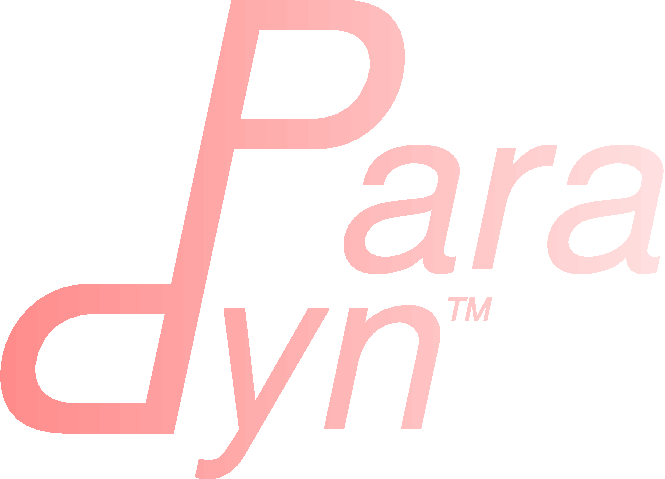
\includegraphics[width=3.25in]{paradyn_logo}
        }; 


\end{tikzpicture}
\endpgfgraphicnamed
\end{titlepage}

\tableofcontents
\clearpage

\section{Introduction}
\label{sec:intro}

A binary code parser converts the machine code representation of a program,
library, or code snippet to abstractions such as the instructions, basic
blocks, and functions that the binary code represents. The ParseAPI is a
multi-platform library for creating such abstractions from binary code sources.
The current incarnation uses the Dyninst SymtabAPI as the default binary code
source; all platforms and architectures handled by the SymtabAPI are supported.
The ParseAPI is designed to be easily extensible to other binary code sources.
Support for parsing binary code in memory dumps or other formats requires only
implementation of a small interface as described in this document.

This API provides the user with a control flow-oriented view of a binary code
source. Each code object such as a program binary or library is represented as
a top-level collection containing the functions, basic blocks, and edges that
represent the control flow graph. A simple query interface is provided for
retrieving lower level objects like functions and basic blocks through address
or other attribute lookups. These objects can be used to navigate the program
structure as described below.

\emph{The ParseAPI is currently released as a public beta. The interfaces
described in this manual are subject to change in future versions. Feedback and
comments are welcome; please email bugs@dyninst.org.}

\section{Abstractions}
\label{sec:abstractions}

The basic representation of code in this API is the control flow
graph (CFG). Binary code objects are represented as regions of contiguous bytes that, when parsed, form the nodes and edges of this graph. The following abstractions make up this CFG-oriented representation of binary code:

% CFG representation abastractions
%
% Function, Block, and Edge
\begin{itemize}[leftmargin=0pt,label=$\circ$]


{\item {\scshape block}: Nodes in the CFG represent \emph{basic blocks}:
straight line sequences of instructions $I_i \ldots I_j$ where for each $i < k
\le j$, $I_k$ postdominates $I_{k-1}$. Importantly, on some instruction set architectures basic blocks can \emph{overlap} on the same address range---variable length instruction sets allow for multiple interpretations of the bytes making up the basic block.
}

{\item {\scshape edge}: Typed edges beween the nodes in the CFG represent
execution control flow, such as conditional and unconditional branches,
fallthrough edges, and calls and returns. The graph therefore represents both
\emph{inter-} and \emph{intraprocedural} control flow: travseral of nodes and
edges can cross the boundaries of the higher level abstractions like
\emph{functions}.
}

{\item {\scshape function}: The \emph{function} is the primary semantic grouping of code in the binary, mirroring the familiar abstraction of procedural languages like C. Functions represent the set of all basic blocks reachable from a \emph{function entry point} through intraprocedural control flow only (that is, no calls or returns). Function entry points are determined in a variety of ways, such as hints from debugging symbols and recursive traversal along call edges.
}

\end{itemize}

% binary code representation abstractions
%
% code object, code source, and instruction source
\begin{itemize}[leftmargin=0pt,label=$\circ$]

{\item {\scshape code object}: A collection of distinct code regions are represented as a single code object, such as an executable or library. Code objects can normally be thought of as a single, discontiguous unique address space. However, the ParseAPI supports code objects in which the different regions have overlapping address spaces, such as UNIX archive files containing unlinked code.
}% end code object

{\item {\scshape instruction source}: An instruction source describes a backing store containing binary code. A binary file, a library, a memory dump or a process's executing memory image can all be described as an instruction source, allowing parsing of a variety of binary code objects.
}% end instruction source

{\item {\scshape code source}: The code source implements the instruction source interface, exporting methods that can access the underlying bytes of the binary code for parsing. It also exports a number of additional helper methods that do things such as returning the location of structured exception handling routines and function symbols. Code sources are tailored to particular binary types; the ParseAPI provides a SymtabAPI-based code source that understands ELF, COFF and PE file formats.
}% end code source

\end{itemize}

\section{A simple example}
\label{sec:example}

The following complete example uses the ParseAPI to parse a binary and dump its control flow graph in the Graphviz file format.

\lstset{language=[GNU]C++,basicstyle=\fontfamily{fvm}\selectfont\small}
\lstset{numbers=left, numberstyle=\tiny, stepnumber=5, numbersep=5pt}
\lstset{showstringspaces=false}
\lstinputlisting{example.cc}

\section{The Parsing API}
\label{sec:api}

\subsection{Class CodeObject}

\definedin{CodeObject.h}

The CodeObject class describes an individual binary code object, such as an
executable or library. It is the top-level container for parsing the object as
well as accessing that parse data. The following API routines and data types
are provided to support parsing and retrieving parsing products.

\begin{apient}
typedef ContainerWrapper<vector<Function*>,Function*,Function*> funclist
\end{apient}
\apidesc{Container for access to functions. Refer to Section \ref{sec:containers} for details. Library users \emph{must not} rely on the underlying container type of ContainerWrapper lists, as it is subject to change.}

\begin{apient}
CodeObject(CodeSource * cs,
    CFGFactory * fact = NULL,
    ParseCallback * cb = NULL,
    bool defensiveMode = false)
\end{apient}
\apidesc{Constructs a new CodeObject from the provided CodeSource and
optional object factory and callback handlers. Any parsing hints provided
by the CodeSource are processed, but the binary is not parsed when this
constructor returns.

\medskip\noindent The \texttt{defensiveMode}
parameter optionally trades off coverage for safety; this mode is not
recommended for most applications as it makes very conservative assumptions
about control flow transfer instructions (see Section \ref{sec:defmode}.}

\begin{apient}
void parse()
\end{apient}
\apidesc{Recursively parses the binary represented by this CodeObject from all
known function entry points (i.e., the hints provided by the CodeSource). This
method and the following parsing methods may safely be invoked repeatedly if
new information about function locations is provided through the CodeSource.}

\begin{apient}
void parse(Address target, bool recursive)
\end{apient}
\apidesc{Parses the binary starting with the instruction at the provided target address. If \texttt{recursive} is {\scshape true}, recursive traversal parsing is used as in the default \texttt{parse()} method; otherwise only instructions reachable through intraprocedural control flow are visited.}

\begin{apient}
void parseGaps(CodeRegion *cr)
\end{apient}
\apidesc{Speculatively parse the indicated region of the binary using pattern matching to find likely function entry points. Only enabled on the x86 32-bit platform.}

\begin{apient}
Function * findFuncByEntry(CodeRegion * cr, Address entry)
\end{apient}
\apidesc{Find the function starting at address \texttt{entry} in the indicated CodeRegion. Returns {\scshape null} if no such function exists.}

\begin{apient}
int findFuncs(CodeRegion * cr, Address addr, std::set<Function*> & funcs)
\end{apient}
\apidesc{Finds all functions spanning \texttt{addr} in the code region, adding each to \texttt{funcs}. The number of results of this stabbing query are returned.}

\begin{apient}
int findFuncs(CodeRegion * cr, Address start, Address end, std::set<Function*> & funcs)
\end{apient}
\apidesc{Finds all functions overlapping the range \texttt{[start,end)} in the code region, adding each to \texttt{funcs}. The number of results of this stabbing query are returned.}

\begin{apient}
funclist & funcs()
\end{apient}
\apidesc{Returns a reference to a container of all functions in the binary. Refer to Section \ref{sec:containers} for container access details.}

\begin{apient}
Block * findBlockByEntry(CodeRegion * cr, Address entry)
\end{apient}
\apidesc{Find the basic block starting at address \texttt{entry}. Returns {\scshape null} if no such block exists.}

\begin{apient}
int findBlocks(CodeRegion * cr, Address addr, std::set<Block*> & blocks)
\end{apient}
\apidesc{Finds all blocks spanning \texttt{addr} in the code region, adding each to \texttt{blocks}. Multiple blocks can be returned only on platforms with variable-length instruction sets (such as IA32) for which overlapping instructions are possible; at most one block will be returned on all other platforms.}

\begin{apient}
void finalize()
\end{apient}
\apidesc{Force complete parsing of the CodeObject; parsing operations are otherwise completed only as needed to answer queries.}

\begin{apient}
CodeSource * cs()
\end{apient}
\apidesc{Return a reference to the underlying CodeSource.}

\begin{apient}
CFGFactory * fact()
\end{apient}
\apidesc{Return a reference to the CFG object factory.}

\subsection{Class CodeSource}
\label{sec:codesource}

\definedin{CodeSource.h}

The CodeSource interface is used by the ParseAPI to retrieve binary code from
an executable, library, or other binary code object; it also can provide hints
of function entry points (such as those derived from debugging symbols) to seed
the parser. The ParseAPI provides a default implementation based on the
SymtabAPI that supports many common binary formats. For details on implementing
a custom CodeSource, see Appendix \ref{sec:extend}.

\begin{apient}
virtual bool nonReturning(Address func_entry)
virtual bool nonReturning(std::string func_name)
\end{apient}
\apidesc{Looks up whether a function returns (by name or location). This information may be statically known for some code sources, and can lead to better parsing accuracy.}

\begin{apient}
virtual Address baseAddress()
virtual Address loadAddress()
\end{apient}
\apidesc{If the binary file type supplies non-zero base or load addresses (e.g. Windows PE), implementations should override these functions.}

\begin{apient}
std::map< Address, std::string > & linkage()
\end{apient}
\apidesc{Returns a reference to the external linkage map, which may or may not be filled in for a particular CodeSource implementation.}

\begin{apient}
std::vector<CodeRegion *> const& regions()
\end{apient}
\apidesc{Returns a read-only vector of code regions within the binary represented by this code source.}

\begin{apient}
int findRegions(Address addr, set<CodeRegion *> & ret)
\end{apient}
\apidesc{Finds all CodeRegion objects that overlap the provided address. Some code sources (e.g. archive files) may have several regions with overlapping address ranges; others (e.g. ELF binaries) do not.}

\begin{apient}
bool regionsOverlap() 
\end{apient}
\apidesc{Indicates whether the CodeSource contains overlapping regions.}

\subsection{Class CodeRegion}

\definedin{CodeSource.h}

The CodeRegion interface is an accounting structure used to divide CodeSources into distinct regions. This interface is mostly of interest to CodeSource implementors.

\begin{apient}
void names(Address addr, vector<std::string> & names)
\end{apient}
\apidesc{Fills the provided vector with any names associated with the function at a given address in the region, e.g. symbol names in an ELF or PE binary.}

\begin{apient}
virtual bool findCatchBlock(Address addr, Address & catchStart)
\end{apient}
\apidesc{Finds the exception handler associated with an address, if one exists. This routine is only implemented for binary code sources that support structured exception handling, such as the SymtabAPI-based SymtabCodeSource provided as part of the ParseAPI.}

\begin{apient}
Address low()
\end{apient}
\apidesc{The lower bound of the interval of address space covered by this region.}

\begin{apient}
Address high()
\end{apient}
\apidesc{The upper bound of the interval of address space covered by this region.}

\begin{apient}
bool contains(Address addr)
\end{apient}
\apidesc{Returns {\scshape true} if $\texttt{addr} \in [\texttt{low()},\texttt{high()})$, {\scshape false} otherwise.}

\subsection{Class Function}

\definedin{CFG.h}

The Function class represents the protion of the program CFG that is reachable through intraprocedural control flow transfers from the function's entry block. Functions in the ParseAPI have only a single entry point; multiple-entry functions such as those found in Fortran programs are represented as several functions that ``share'' a subset of the CFG. 

\begin{center}
\begin{tabular}{ll}
\toprule
FuncSource & Meaning \\
\midrule
RT & recursive traversal (default) \\
HINT & specified in CodeSource hints \\
GAP & speculative parsing heuristics \\
GAPRT & recursive traversal from speculative parse \\
ONDEMAND & dynamically discovered at runtime \\
\bottomrule
\end{tabular}
\end{center}

\apidesc{Return type of function \texttt{src()} see description below.}

\begin{center}
\begin{tabular}{ll}
\toprule
FuncReturnStatus & Meaning \\
\midrule
UNSET & unparsed function (default) \\
NORETURN & will not return \\
UNKNOWN & cannot be determined statically \\
RETURN & may return \\
\bottomrule
\end{tabular}
\end{center}

\apidesc{Return type of function \texttt{retstatus()}, see description below.}

\begin{apient}
typedef ContainerWrapper<vector<Block*>,Block*,Block*> blocklist
typedef ContainerWrapper<vector<Edge*>,Edge*,Edge*> edgelist
\end{apient}
\apidesc{Containers for block and edge access. Refer to Section \ref{sec:containers} for details on \texttt{ContainerWrapper}. Library users \emph{must not} rely on the underlying container type of ContainerWrapper lists, as it is subject to change.}

\begin{apient}
const string & name()
\end{apient}
\apidesc{Returns the name of this function.}

\begin{apient}
CodeRegion * region()
\end{apient}
\apidesc{Returns the CodeRegion that contains this function's entry point (functions can span multiple regions).}

\begin{apient}
InstructionSource * isrc()
\end{apient}
\apidesc{Returns the InstructionSource for this function.}

\begin{apient}
CodeObject * obj()
\end{apient}
\apidesc{Returns the CodeObject containing this function.}

\begin{apient}
FuncSource src()
\end{apient}
\apidesc{Returns the type of hint that identified this function's entry point.}

\begin{apient}
FuncReturnStatus retstatus()
\end{apient}
\apidesc{Returns the best-effort determination of whether this function may return or not. Return status cannot always be statically determined, and at most can guarantee that a function \emph{may} return, not that it \emph{will} return.}

\begin{apient}
Block * entry()
\end{apient}
\apidesc{Returns the basic block at this function's entry point.}

\begin{apient}
bool parsed()
\end{apient}
\apidesc{Indicates whether this function has been parsed.}

\begin{apient}
blocklist & blocks()
\end{apient}
\apidesc{Returns a list of the basic blocks comprised by this function. The blocks are guaranteed to be sorted by starting address.}

\begin{apient}
bool contains(Block *b)
\end{apient}
\apidesc{Returns {\scshape true} if the block is contained in this function.}

\begin{apient}
edgelist & callEdges()
\end{apient}
\apidesc{Returns a list of all outgoing call edges from this function.}

\begin{apient}
blocklist & returnBlocks()
\end{apient}
\apidesc{Returns a list of all blocks ending in a \texttt{return} instruction.}

\begin{apient}
std::vector<FuncExtent *> const& extents()
\end{apient}
\apidesc{Returns a list of contiguous extents of binary code within the function.}

[The following methods provide additional details about functions to support instrumentation applications and are probably of no interest to most users.]

\begin{apient}
bool hasNoStackFrame()
\end{apient}
\apidesc{Indicates whether the function sets up a stack frame.}

\begin{apient}
bool savesFramePointer()
\end{apient}
\apidesc{Indicates whether the function saves a stack frame pointer.}

\begin{apient}
bool cleansOwnStack()
\end{apient}
\apidesc{Indicates whether the function tears down its own stack on return.}

\subsection{Class FuncExtent}

\definedin{CFG.h}

Function Extents are used internally for accounting and lookup purposes. They may be useful for users who wish to precisely identify the ranges of the address space spanned by functions (functions are often discontiguous, particularly on architectures with variable length instruction sets).

\begin{apient}
Address start()
\end{apient}
\apidesc{The start of this contiguous code extent.}

\begin{apient}
Address end()
\end{apient}
\apidesc{The end of this contiguous code extent (exclusive).}

\subsection{Class Block}

\definedin{CFG.h}

A Block represents a basic block as defined in Section \ref{sec:abstractions}, and is the lowest level representation of code in the CFG.

\begin{apient}
typedef ContainerWrapper<vector<Edge*>,Edge*,Edge*> edgelist
\end{apient}
\apidesc{Container for edge access. Refer to Section \ref{sec:containers} for details. Library users \emph{must not} rely on the underlying container type of ContainerWrapper lists, as it is subject to change.}


\begin{apient}
Address start()
\end{apient}
\apidesc{Returns the lower bound of this block (the address of the first instruction).}

\begin{apient}
Address end()
\end{apient}
\apidesc{Returns the upper bound (open) of this block (the address immediately
following the last byte in the last instruction). }

\begin{apient}
Address lastInsnAddr()
\end{apient}
\apidesc{Returns the address of the last instruction in this block.}

\begin{apient}
Address size()
\end{apient}
\apidesc{Returns $\texttt{end()} - \texttt{start()}$.}

\begin{apient}
bool parsed()
\end{apient}
\apidesc{Indicates whether this block has been parsed.}

\begin{apient}
CodeObject * obj()
\end{apient}
\apidesc{Returns the CodeObject containing this block.}

\begin{apient}
CodeRegion * region()
\end{apient}
\apidesc{Returns the CodeRegion containing this block.}

\begin{apient}
edgelist & sources()
\end{apient}
\apidesc{Return a list of all incomming edges to the block.}

\begin{apient}
edgelist & targets()
\end{apient}
\apidesc{Return a list of all outgoing edges from the block.}

\begin{apient}
bool consistent(Address addr, Address & prev_insn)
\end{apient}
\apidesc{Check whether address \texttt{addr} is \emph{consistent} with this basic block. An address is consistent if it is the boundary between two instructions in the block. As long as \texttt{addr} is within the range of the block, \texttt{prev\_insn} will contain the address of the previous instruction boundary before \texttt{addr}, regardless of whether \texttt{addr} is consistent or not.}

\begin{apient}
int containingFuncs()
\end{apient}
\apidesc{Returns the number of functions that contain this block.}

\begin{apient}
void getFuncs(std::vector<Function *> & funcs)
\end{apient}
\apidesc{Fills in the provided vector with all functions that share this basic block.}

\subsection{Class Edge}

\definedin{CFG.h}

Typed Edges join two blocks in the CFG, indicating the type of control flow
transfer instruction that joins the blocks to each other. Edges may not correspond
to a control flow transfer instruction at all, as in the case of the {\scshape
fallthrough} edge that indicates where straight-line control flow is split by
incoming transfers from another location, such as a branch. While not all
blocks end in a control transfer instruction, all control transfer instructions
end basic blocks and have outgoing edges; in the case of unresolvable control
flow, the edge will target a special ``sink'' block (see \texttt{sinkEdge()},
below.

\begin{center}
\begin{tabular}{ll}
\toprule
EdgeTypeEnum & Meaning \\
\midrule
CALL & call edge \\
COND\_TAKEN & conditional branch--taken \\
COND\_NOT\_TAKEN & conditional branch--not taken \\
INDIRECT & branch indirect \\
DIRECT & branch direct \\
FALLTHROUGH & direct fallthrough (no branch) \\
CATCH & exception handler \\
CALL\_FT & post-call fallthrough \\
RET & return \\
\bottomrule
\end{tabular}
\end{center}

\begin{apient}
Block * src()
\end{apient}
\apidesc{Returns the source block of this edge.}

\begin{apient}
Block * trg()
\end{apient}
\apidesc{Returns the target block of this edge.}

\begin{apient}
EdgeTypeEnum type()
\end{apient}
\apidesc{Returns the edge type.}

\begin{apient}
bool sinkEdge()
\end{apient}
\apidesc{Indicates whether this edge targets the special \emph{sink} block.}

\begin{apient}
bool interproc()
\end{apient}
\apidesc{Returns {\scshape true} if the edge should be interpreted as interprocedural (e.g. calls, returns, direct branches under certain circumstances).}

\subsection{Class EdgePredicate}
\label{sec:pred}

\definedin{CFG.h}

Edge predicates control iteration over edges. For example, the provided
\texttt{Intraproc} edge predicate can be passed to an edge iterator
constructor, ensuring that only intraprocedural edges are visited during
iteration. Two other implementations of EdgePredicate are provided: 
\texttt{SingleContext} only visits edges that stay in a single
function context, and \texttt{NoSinkPredicate} does not visit edges to 
the \emph{sink} block.  The following code traverses 
all of the basic blocks within a
function:

\lstset{language=[GNU]C++,basicstyle=\fontfamily{fvm}\selectfont\small}
\lstset{numbers=left, numberstyle=\tiny, stepnumber=5, numbersep=5pt}
\begin{lstlisting}
    vector<Block*> work;
    std::map<Block*,bool> seen; // avoid loops
    Intraproc epred; // ignore calls, returns
   
    work.push_back(func->entry()); // assuming `func' is a Function*
    seen[func->entry()] = true;
    while(!work.empty()) {
        Block * b = work.back();
        work.pop_back();

        // do some stuff with b...
   
        Block::edgelist & targets = block->targets();
        Block::edgelist::iterator eit = targets.begin(&epred);
        for( ; eit != targets.end(); ++eit) {
            Edge * e = (*eit);
            if(seen.find(e->trg()) == seen.end())
                work.push_back(e->trg());
        }
    } 
\end{lstlisting}

New edge predicates can be created by implementing the following simple interface:

\begin{apient}
EdgePredicate()
EdgePredicate(EdgePredicate * next)
\end{apient}
\apidesc{Constructs a predicate, either with or without a previously existing predicate to chain it to. Chained predicates return the logical AND over all predicates in the chain.}

\begin{apient}
virtual bool pred_impl(Edge *)
\end{apient}
\apidesc{Evaluates the predicate on the provided edge.}

\subsection{Class ParseCallback}

\definedin{ParseCallback.h}

The ParseCallback class allows ParseAPI users to be notified of various events
during parsing. For most users this notification is unnecessary, and an
instantiation of the default ParseCallback can be passed to the CodeObject during initialization. Users who wish to be notified must implement a class that inherits from ParseCallback, and implement one or more of the methods described below to receive notification of those events.

\begin{apient}
struct default_details {
    default_details(unsigned char*b,size_t s, bool ib) : ibuf(b), isize(s), isbranch(ib) { }
    unsigned char * ibuf;
    size_t isize;
    bool isbranch;
}
\end{apient}
\apidesc{Details used in the \texttt{unresolved\_cf} and \texttt{abruptEnd\_cf}
callbacks.}

\begin{apient}
virtual void instruction_cb(Function*,Address,insn_details*)
\end{apient}
\apidesc{Invoked for each instruction decoded during parsing. Implementing this callback may incur significant overhead.}

\begin{apient}
struct insn_details {
    InsnAdapter::InstructionAdapter * insn;
}
\end{apient}

\begin{apient}
void interproc_cf(Function*,Address,interproc_details*)
\end{apient}
\apidesc{Invoked for each interprocedural control flow instruction.}

\begin{apient}  
struct interproc_details {
    typedef enum {
        ret,
        call,
        branch_interproc, // tail calls, branches to plts
        syscall
    } type_t;
    unsigned char * ibuf;
    size_t isize;
    type_t type;
    union {
        struct {
            Address target;
            bool absolute_address;
            bool dynamic_call;
        } call;
    } data;
}
\end{apient}
\apidesc{Details used in the \texttt{interproc\_cf} callback.}

\begin{apient}
void overlapping_blocks(Block*,Block*)
\end{apient}
\apidesc{Noification of inconsistent parse data (overlapping blocks).}

\subsection{Containers}
\label{sec:containers}

Several of the ParseAPI data structures export containers of CFG objects; the
CodeObject provides a list of functions in the binary, for example, while
functions provide lists of blocks and so on. To avoid tying the internal
storage for these structures to any particular container type, ParseAPI objects
export a ContainerWrapper that provides an iterator interface to the internal
containers. These wrappers and predicate interfaces are designed to add minimal
overhead while protecting ParseAPI users from exposure to internal container
storage details. Users \emph{must not} rely on properties of the underlying
container type (e.g. storage order) unless that property is explicity stated in
this manual.

\noindent
ContainerWrapper containers export the following interface (\texttt{iterator} types vary depending on the template parameters of the ContainerWrapper, but are always instantiations of the PredicateIterator described below):

\begin{apient}
iterator begin()
iterator begin(predicate *)
\end{apient}
\apidesc{Return an iterator pointing to the beginning of the container, with or without a filtering predicate implementation (see Section \ref{sec:pred} for details on filter predicates).}

\begin{apient}
iterator const& end()
\end{apient}
\apidesc{Return the iterator pointing to the end of the container (past the last element).}

\begin{apient}
size_t size()
\end{apient}
\apidesc{Returns the number of elements in the container. Execution cost may vary depending on the underlying container type.}

\begin{apient}
bool empty()
\end{apient}
\apidesc{Indicates whether the container is empty or not.}

\noindent
The elements in ParseAPI containers can be accessed by iteration using an instantiation of the PredicateIterator. These iterators can optionally act as filters, evaluating a boolean predicate for each element and only returning those elements for which the predicate returns {\scshape true}. \emph{Iterators with non-{\scshape null} predicates may return fewer elements during iteration than their \texttt{size()} method indicates.} Currently PredicateIterators only support forward iteration. The operators \texttt{++} (prefix and postfix), \texttt{==}, \texttt{!=}, and \texttt{*} (dereference) are supported.


\appendix
\section{Extending ParseAPI}
\label{sec:extend}

The ParseAPI is design to be a low level toolkit for binary analysis tools.
Users can extend the ParseAPI in two ways: by extending the control flow
structures (Functions, Blocks, and Edges) to incorporate additional data to
support various analysis applications, and by adding additional binary code
sources that are unsupported by the default SymtabAPI-based code source. For
example, a code source that represents a program image in memory could be
implemented by fulfilling the CodeSource and InstructionSource interfaces
described in Section \ref{sec:codesource} and below. Implementations that
extend the CFG structures need only provide a custom allocation factory in
order for these objects to be allocated during parsing.

\subsection{Instruction and Code Sources}

A CodeSource, as described above, exports its own and the InstructionSource interface for access to binary code and other details. In addition to implementing the virtual methods in the CodeSource base class (Section \ref{sec:codesource}), the methods in the pure-virtual InstructionSource class must be implemented:

\begin{apient}
virtual bool isValidAddress(const Address) 
\end{apient}
\apidesc{Returns {\scshape true} if the address is a valid code location.}

\begin{apient}
virtual void* getPtrToInstruction(const Address)
\end{apient}
\apidesc{Returns pointer to raw memory in the binary at the provided address.}

\begin{apient}
virtual void* getPtrToData(const Address)
\end{apient}
\apidesc{Returns pointer to raw memory in the binary at the provided address. The address need not correspond to an executable code region.}

\begin{apient}
virtual unsigned int getAddressWidth()
\end{apient}
\apidesc{Returns the address width (e.g. four or eight bytes) for the represented binary.}

\begin{apient}
virtual bool isCode(const Address)
\end{apient}
\apidesc{Indicates whether the location is in a code region.}

\begin{apient}
virtual bool isData(const Address)
\end{apient}
\apidesc{Indicates whether the location is in a data region.}

\begin{apient}
virtual Address offset()
\end{apient}
\apidesc{The start of the region covered by this instruction source.}

\begin{apient}
virtual Address length()
\end{apient}
\apidesc{The size of the region.}

\begin{apient}
virtual Architecture getArch()
\end{apient}
\apidesc{The architecture of the instruction source. See the Dyninst manual for details on architecture differences.}

\begin{apient}
virtual bool isAligned(const Address)
\end{apient}
\apidesc{For fixed-width instruction architectures, must return {\scshape true} if the address is a valid instruction boundary and {\scshape false} otherwise; otherwise returns {\scshape true}. This method has a default implementation that should be sufficient.}

CodeSource implementors need to fill in several data structures in the base CodeSource class:

\begin{apient}
std::map<Address, std::string> _linkage
\end{apient}
\apidesc{Entries in the linkage map represent external linkage, e.g. the PLT in ELF binaries. Filling in this map is optional.}

\begin{apient}
Address _table_of_contents
\end{apient}
\apidesc{Many binary format have ``table of contents'' structures for position
independant references. If such a structure exists, its address should be filled in.}

\begin{apient}
std::vector<CodeRegion *> _regions
Dyninst::IBSTree<CodeRegion> _region_tree
\end{apient}
\apidesc{One or more contiguous regions of code or data in the binary object must be registered with the base class. Keeping these structures in sync is the responsibility of the implementing class.}

\begin{apient}
std::vector<Hint> _hints
\end{apient}
\apidesc{CodeSource implementors can supply a set of Hint objects describing where functions are known to start in the binary. These hints are used to seed the parsing algorithm. Refer to the CodeSource header file for implementation details.}

\subsection{CFG Object Factories}
\label{sec:factories}

Users who which to incorporate the ParseAPI into large projects may need to store additional information about CFG objects like Functions, Blocks, and Edges. The simplest way to associate the ParseAPI-level CFG representation with higher-level implementation is to extend the CFG classes provided as part of the ParseAPI. Because the parser itself does not know how to construct such extended types, implementors must provide an implementation of the CFGFactory that is specialized for their CFG classes. The CFGFactory exports the following simple interface:

\begin{apient}
virtual Function * mkfunc(Address addr, 
    FuncSource src,
    std::string name, 
    CodeObject * obj, 
    CodeRegion * region,
    Dyninst::InstructionSource * isrc)
\end{apient}
\apidesc{Returns an object derived from Function as though the provided parameters had been passed to the Function constructor. The ParseAPI parser will never invoke \texttt{mkfunc()} twice with identical \texttt{addr}, and \texttt{region} parameters---that is, Functions are guaranteed to be unique by address within a region.}

\begin{apient}
virtual Block * mkblock(Function * func, CodeRegion * region, Address addr)
\end{apient}
\apidesc{Returns an object derived from Block as though the provided parameters had been passed to the Block constructor. The parser will never invoke \texttt{mkblock()} with identical \texttt{addr} and \texttt{region} parameters.}

\begin{apient}
virtual Edge * mkedge(Block * src, Block * trg, EdgeTypeEnum type)
\end{apient}
\apidesc{Returns an object derived from Edge as though the provided parameters had been passed to the Edge constructor. The parser \emph{may} invoke \texttt{mkedge()} multiple times with identical parameters.}

\begin{apient}
virtual Block * mksink(CodeObject *obj, CodeRegion *r)
\end{apient}
\apidesc{Returns a ``sink'' block derived from Block to which all unresolvable control flow instructions will be linked. Implementors may return a unique sink block per CodeObject or a single global sink.}

Implementors of extended CFG classes are required to override the default implementations of the \emph{mk*} functions to allocate and return the appropriate derived types statically cast to the base type. Implementors must also add all allocated objects to the following internal lists:

\begin{apient}
fact_list<Edge> edges_
fact_list<Block> blocks_
fact_list<Function> funcs_
\end{apient}
\apidesc{O(1) allocation lists for CFG types. See the CFG.h header file for list insertion and removal operations.}

Implementors \emph{may} but are \emph{not required to} override the
deallocation following deallocation routines. The primary reason to override
these routines is if additional action or cleanup is necessary upon CFG object
release; the default routines simply remove the objects from the allocation
list and invoke their destructors.

\begin{apient}
virtual void free_func(Function * f)
virtual void free_block(Block * b)
virtual void free_edge(Edge * e)
virtual void free_all()
\end{apient}
\apidesc{CFG objects should be freed using these functions, rather than delete, to avoid leaking memory.}

\section{Defensive Mode Parsing}
\label{sec:defmode}

Binary code that defends itself against analysis may violate the
assumptions made by the the ParseAPI's standard parsing algorithm.
Enabling defensive mode parsing activates more conservative
assumptions that substantially reduce the percentage of code that is
analyzed by the ParseAPI.  For this reason, defensive mode parsing is
best-suited for use of ParseAPI in conjunction with dynamic analysis
techniques that can compensate for its limited coverage of the binary
code.  This mode of parsing will be brought to full functionality in 
an upcoming release.  

\end{document}
